\section{様々な系外惑星スペクトル}



図\ref{fig:earth}は地球のスペクトルである。地球の場合、大気が薄いので輻射光はほぼ放射平衡温度に近い黒体となっている。また反射スペクトルは恒星スペクトルに大気吸収がかかったものとなっている。

図\ref{fig:bd}は褐色矮星のスペクトル。黒体から大きく外れている。

図\ref{fig:jwst}はJWST NIRSPECによるホットサターンWASP-39bのスペクトルである。分子吸収によるfeatureが見て取れる。


\begin{figure}[]
 \begin{center}
	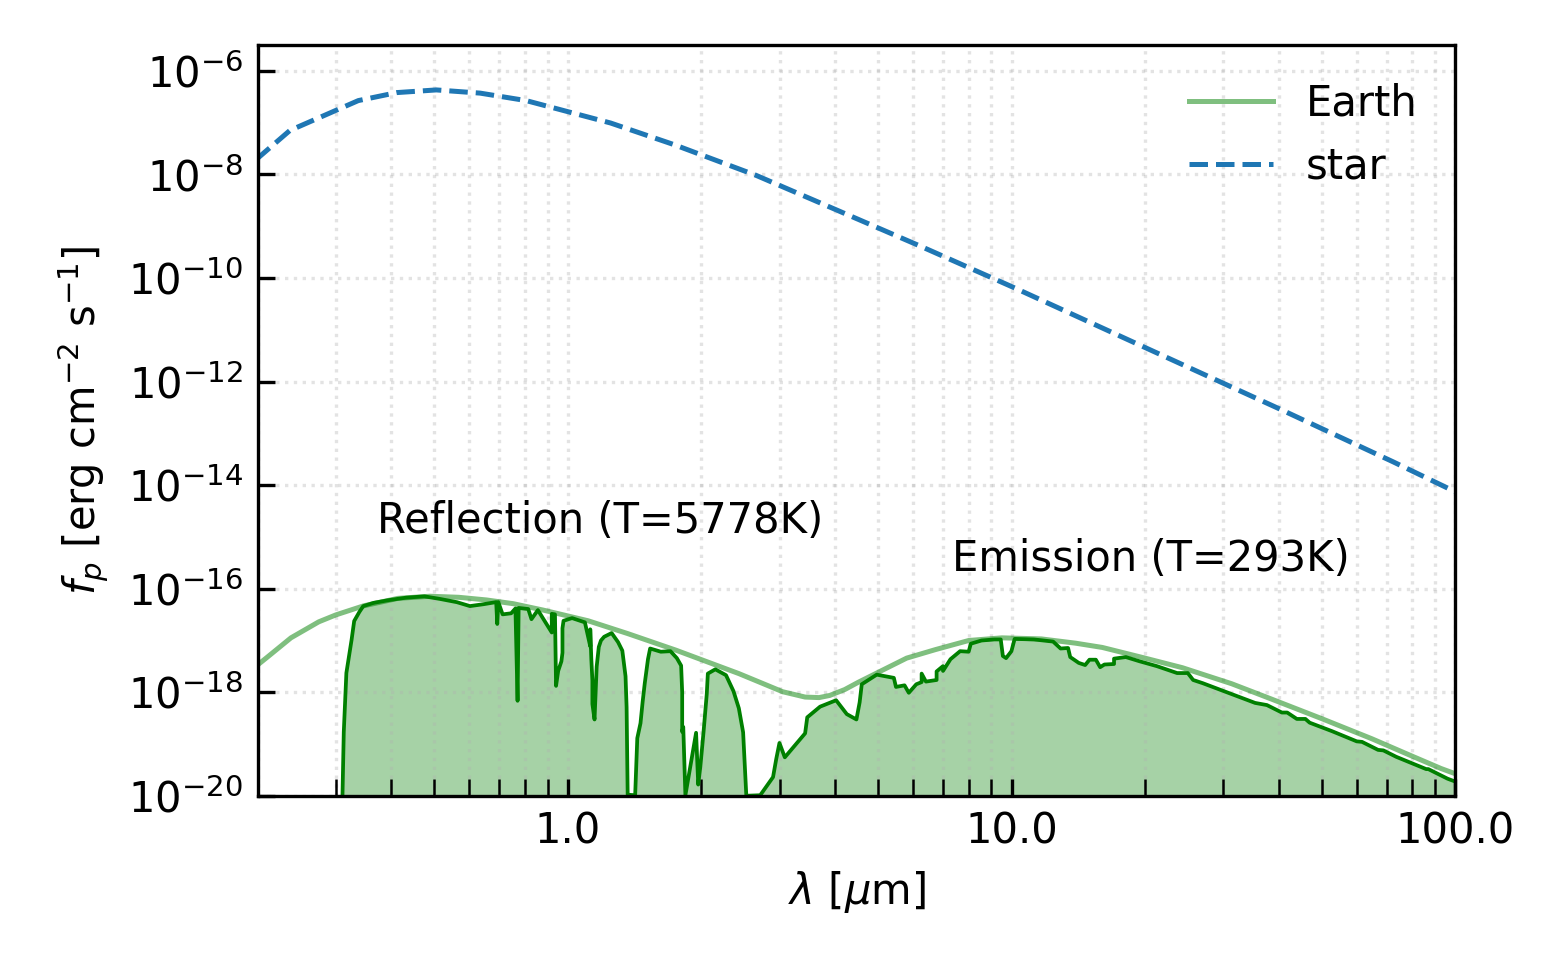
\includegraphics[width=\linewidth]{fig/EarthEmis.png}
\end{center}
	\caption{地球のスペクトル}
	\label{fig:earth}
\end{figure} 

\begin{figure}[]
 \begin{center}
	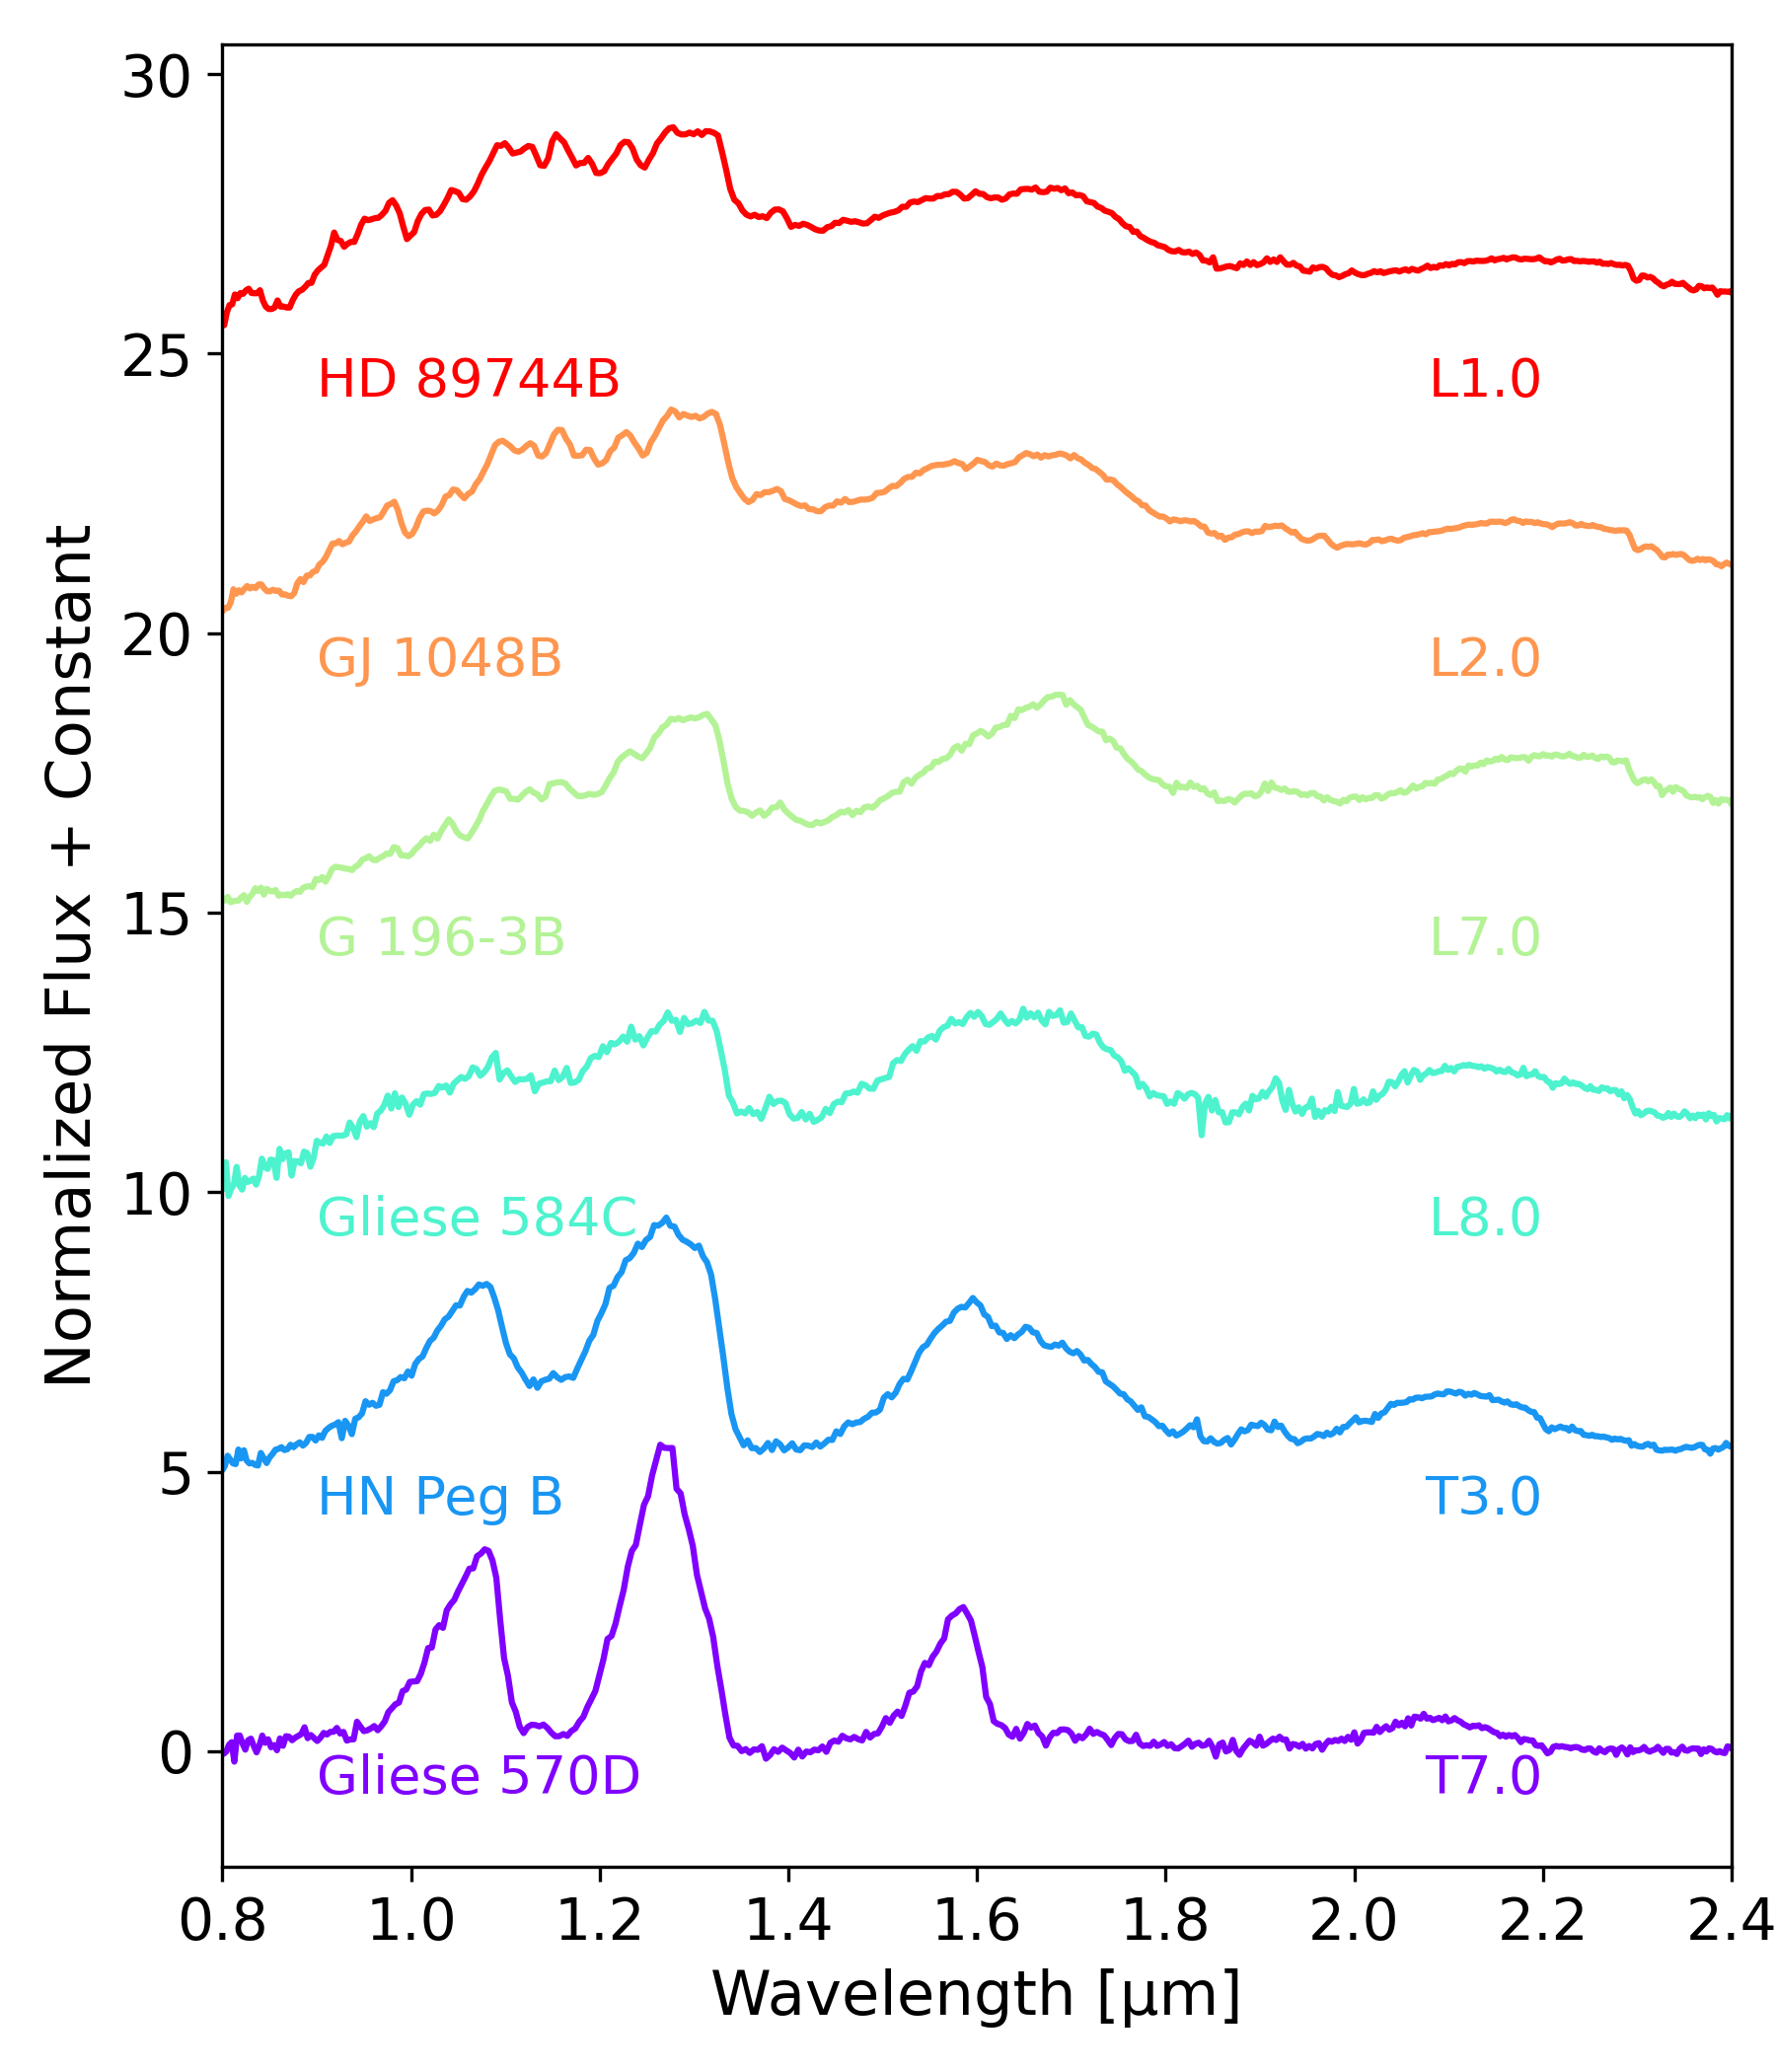
\includegraphics[width=\linewidth]{fig/bdspectra.png}
\end{center}
	\caption{褐色矮星のスペクトル (SpeX Prismライブラリー) Inspired by\cite{2025ApJ...988...31L}}
	\label{fig:bd}
\end{figure} 


\begin{figure*}[htb]
 \begin{center}
	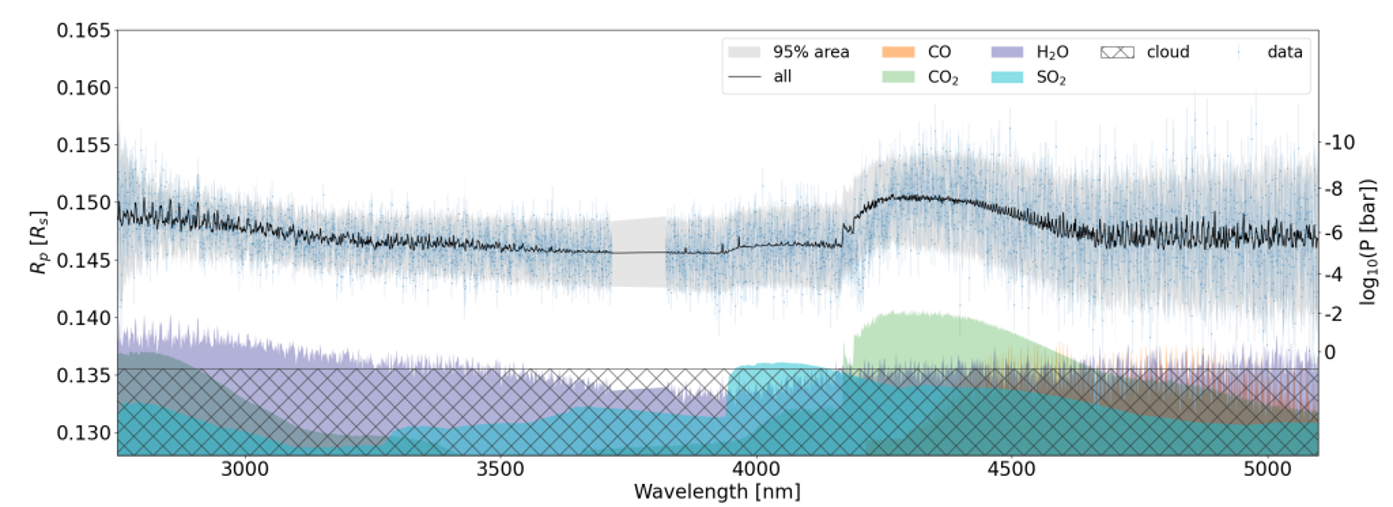
\includegraphics[width=\linewidth]{fig/jwst_spectrum.png}
\end{center}
	\caption{JWST透過光スペクトル WASP-39 b \cite{2025ApJ...985..263K}}
	\label{fig:jwst}
\end{figure*} 


